\section{Anwendungsszenarien}%Graph-Datenbanken - Grundlegende technologische Aspekte (chapter)
\subsection{Text-Mining, Natural Language Processing}
Im Fachgebiet des Text Minings, oder auch des Natural Language Processing (NLP), geht es um die Extraktion, Interpretation und statistische Auswertung von natürlich-menschlicher Sprache. Entsprechende Verfahren des NLP ermöglichen es, Informationen aus Texten zu extrahieren. Auch das Erkennen von Wortarten von Wörtern innerhalb eines Satzes spielt dabei eine Rolle.

Seit der Entwicklung von Smartphones gewann das NLP an Bedeutung. So wurden Verfahren der \emph{Tippkorrektur} implementiert und kommen auf zahlreichen Smartphones zum Einsatz. Inzwischen wurde die Tippkorrektur auch um eine Funktion der \emph{Autovervollständigung} erweitert, bei der Wörter nach der Eingabe von nur wenigen Buchstaben zur Vervollständigung vorgeschlagen werden. Anhand der Beobachtung welche Wörter besonders häufig miteinander vorkommen, schlagen Verfahren zur Autovervollständigung oft sogar ganze Wörter oder gar Reihen von Worten vor, ohne das damit begonnen wurde sie einzutippen. Auch bei der Übersetzung von Sätzen in eine andere Sprache kommen Verfahren des NLP zum Einsatz.

Zur Vorhersage von Wörtern oder Buchstaben werden mitunter Hidden-Markov-Modelle zur Hilfe gezogen \cite[p.~207]{jurafsky01}. Bei Hidden-Markov-Modellen handelt es sich um ein sehr wichtiges Verfahren des Machine-Learnings. Bei Markov-Ketten handelt es sich um gewichtete, endliche Automaten. Die Markov-Kette besteht auch Knoten, die mittels gewichteter Kanten miteinander verbunden sind. Die Knoten stellen hierbei einen Zustand, wie beispielsweise ein Wort, dar. Die gewichteten Kanten beschreiben die Wahrscheinlichkeit, dass der jeweils nächste Zustand eintritt \cite[p.~208 ff.]{jurafsky01}\cite[p.~318 ff.]{manning01}. Bei einem Hidden-Markov-Modell wird zwischen beobachtbaren und versteckten Zuständen unterschieden. Es handelt sich hierbei um eine Erweiterung von Markov-Ketten \cite[p.~211 ff.]{jurafsky01}. 

Markov-Modelle werden durch Verfahren des Machine-Learnings gebildet. Dabei werden Trainingsdaten benötigt, aus denen die Wahrscheinlichkeit für bestimmte Zustände ermittelt werden. Für das Anlernen der Wahrscheinlichkeiten und der Zustände gibt es unterschiedliche Verfahren \cite[p.~213 ff.]{jurafsky01}\cite[p.~326 ff.]{manning01}. Grundsätzlich lässt sich festhalten, dass die Aussagekraft eines Markov-Modells in Abhängigkeit zur Trainingsmenge steht. Eine hohe Aussagekraft des Modells wird mit einer großen Trainingsmenge erreicht. Jedoch steigt mit einer größeren Trainingsmenge auch der Aufwand des jeweiligen Lernverfahrens.

Bei Markov-Ketten handelt es sich um gewichtete Graphen, deren Umsetzung sich in einer Graph-Datenbank anbietet. Auf diese Weise kann auf einer für Graphen natürlichen Art und Weise ein Ergebnis für die Markov-Kette berechnet werden. Graph-Datenbanken, die die jeweiligen Markov-Modelle beinhalten, können dann auf anderen Geräten, wie Computer, Server oder Smartphones, gespeichert und dort genutzt werden. So werden unter Anderem Systeme zur Tippfehlerkorrektur unterstützt. Durch die Übertragung von Markov-Modellen in Graph-Datenbanken ist es also möglich, bereits trainierte Modelle auf andere Computer zu übertragen und dort nutzbar zu machen. Auf diese Weise müssen Markov-Modelle auf den Computersystemen, auf denen sie genutzt werden sollen, nicht erst trainiert werden.

\subsection{Soziale Netze}
Unter dem Begriff Sozialem Netz versteht man eine Menge an Teilnehmern, häufig sind dies natürliche Personen, und verschiedenen Arten an Relationen zwischen diesen. Das durch die Beziehungen gebildete Netz lässt sich problemlos als Graph darstellen, indem die Teilnehmer als Knoten des Graphen dargestellt und die Beziehungen auf die Kanten abgebildet werden.

\begin{figure}[h]
	\caption{Auschnitt aus Facebooks Socail-Graph: Checkin \cite{facebookTao}}
	\label{fig:fbCheckin}
	\centering
	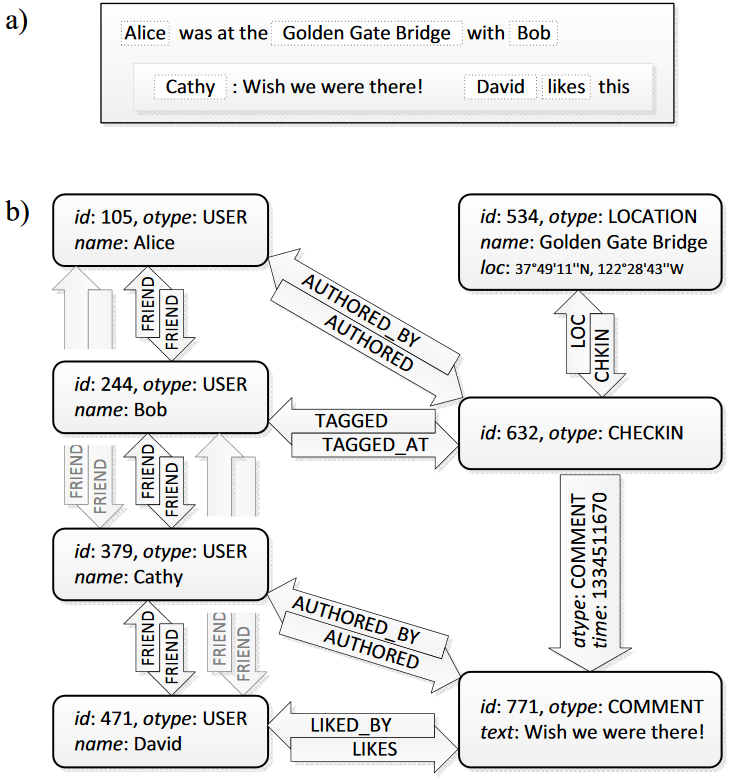
\includegraphics[width=0.7\textwidth]{images/facebook_checkin.png}
\end{figure}

Abbildung~\ref{fig:fbCheckin} zeigt beispielhaft wie ein Teil des Sozialen Netzes von Facebook aussieht. Anhand solcher Einträge wird für jeden einzelnen Nutzer eine personalisierte Startseite in Echtzeit erzeugt, dementsprechend wichtig ist ein performanter Datenzugriff. Um den Anforderungen gerecht zu werden hat Facebook eine eigene Graph-ähnliche API namens TAO entwickelt, welche den Datenbankzugriff effizient steuert. TAO stellt minimale Create/Update/Delete-Kommandos für Knoten und Kanten bereit. Der Großteil der Datenbankzugriffe ist allerdings lesend, folgende Querys sind möglich \cite{facebookTao}:
\begin{itemize}
	\item Alle Assoziation eines Typs zu einem Knoten
	\item Anzahl der Assoziationen eines Typs an einem Knoten
	\item Alle Nachbarn bis zur Tiefe n über eine bestimmte Assoziation
\end{itemize}

Mittels mathematischer Verfahren wie Zentralitätsberechnung, Dichte und Cliquenanalyse können für den Nutzer relevante Beiträge bestimmt werden \cite{sozialeNetzwerkanalyse}. Die für diese Berechnung benötigten Daten werden typischerweise in der Form von Graphen dargestellt. Mittels der zuvor beschrieben API können diese effizient und schnell aus der Datenbank geladen werden.


\subsection{Betrugserkennung}
Graphdatenbanken werden auch im E-Commerce genutzt um Betrug zu vermeiden. Durch die Analyse diverser Pattern lassen sich Betrugsversuche identifizieren und unterbinden noch bevor ernsthafte Schäden entstehen. Analyse der Pattern können durch Trigger ausgelöst werden, diese sind beispielsweise: Einloggen in das System, Registrierung einer neuen Bankkarte oder Bestellung von Waren.

\begin{figure}[h]
	\caption{Serien von den Transaktionen \cite{Betrugserkennung}}
	\label{fig:Trs}
	\centering
	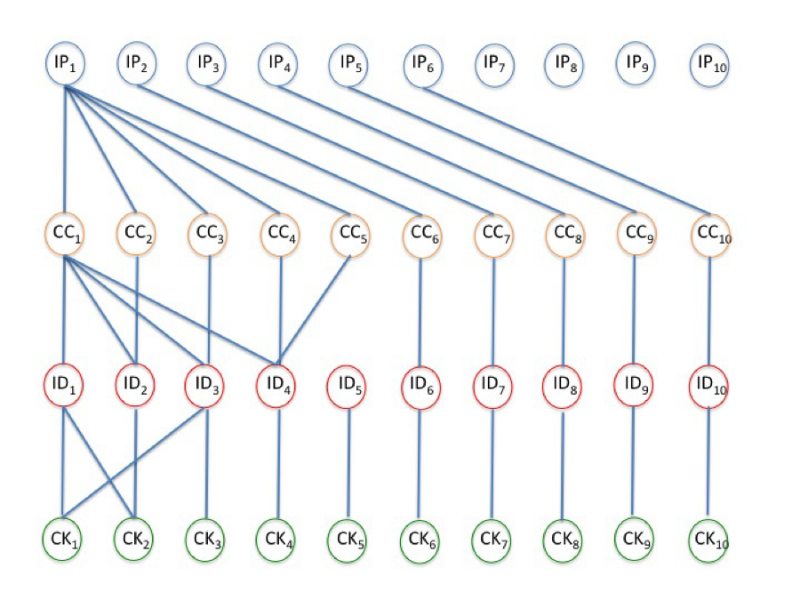
\includegraphics[width=0.7\textwidth]{images/Betrugserkennung.png}
\end{figure}

Auf Abbildung~\ref{fig:Trs} sind Transaktionsserien ausgehend von verschiedenen IP Adressen dargestellt. [IP(x) - IP Adresse, CC(x) - die Kreditkartennummer, ID(x) - der Nutzeraccount, CK(x) - im Browser gespeichertes Cookie]. In diesem Beispiel ist davon auszugehen, dass hinter IP(1) Betrüger stehen. Denn von dem Rechner mit der IP(1) wurden viele Transaktionen mit den unterschiedlichen Kreditkarten durchgeführt. Des weiteren wurde eine Kreditkarte von mehreren Nutzer verwendet auch die Cookies überschneiden sich mit den Accounts. \cite{Betrugserkennung}

Aufgrund der zahlreichen Assoziationen sind Graphdatenbanken ideal für mathematische Lösungsstrategien bei der Erkennung von Betrugsversuchen, damit spielen diese eine wichtige Rolle bei der Finanzsicherheit im Netz.

\subsection{Empfehlungssysteme}
Empfehlungsalgorithmen analysieren die Beziehungen zwischen den Personen und Objekten (z.B. Waren, Dienstleistungen, Medieninhalte). Die Arten der Beziehungen sind vielfältig und vom Business Case getrieben, typisch sind Käufe oder Bewertungen von ähnlichen Objekten.

Die Effektivität der Empfehlungen korreliert mit dem Verständnis über die Beziehungen zwischen den Objekten, sowie der Qualität und Stärke der Verbindung. Diese Struktur lässt sich am besten in Form von den attribuierten Graphen darstellen. Anfragen auf den Graphen sind sehr oft lokal, weil ihre Startpunkte nur wenige identifizierte Objekte sind. Bei der Suche nach Empfehlungen wird nur in der unmittelbaren Nähe von dieser Objekten gesucht.

Eine der ersten Empfehlungssysteme war das System des Internetversandhändlers Amazon. Google entwickelte ein noch fortschrittlicheres System welches erstmal erweiterte Nutzerinformationen verwendet. Bei dem Besuch von Webseiten werden mittels Cookies Informationen über den Nutzer und sein Surfverhalten zusammengetragen. Anhand dieser Daten wird ein Nutzerprofil erstellt welches in die Suchergebnisse von Google einfließt. 
\cite[p.~107]{GraphDB}

\subsection{Verkehrsnetze}
Im öffentlichen Leben spielen Verkehrsnetze eine wichtige Rolle. So kann der öffentliche Nahverkehr als ein Verkehrsnetz betrachtet werden. Die unterschiedlichen Linien und Haltestellen sind Bestandteil des öffentlichen Nahverkehrs und dienen dazu, Menschen zu transportieren. Jedoch ist es mit steigender Komplexität des Verkehrsnetzes und des Taktes nicht immer einfach, den kürzesten und schnellsten Weg zu finden.

Außerdem lässt sich auch der normale Straßenverkehr als Verkehrsnetz begreifen. Die zahlreichen Straßen bilden ein Netz, welches durch ein Auto flexibel genutzt werden kann. Das Straßen-Verkehrsnetz ist dabei recht kompliziert, so dass es auch hier schwer ist, den besten Weg vom Start- zum Zielort zu finden.

Verkehrsnetze lassen sich als Graphen darstellen. Am Beispiel des öffentlichen Nahverkehrs können Haltestellen als Knoten, sowie die Strecken zwischen den Haltestellen als Kanten bezeichnet werden. Kanten können darüber hinaus gerichtet sein, um die unterschiedlichen Richtungen einer Linie abzubilden. \cite[p.~74 ff.]{bartelme01}

Dabei müssen Graphen für das Verkehrsnetz des öffentlichen Nahverkehrsnetz nicht zwangsläufig die tatsächliche Straßenverkehrsführung wiedergeben. Wenn beispielsweise eine Straße gesperrt wird und ein Autobus eine Umleitung fahren muss, bleiben die Knoten-Kanten-Beziehungen, sofern keine Haltestellen ausfallen und hinzukommen. Auf diese Weise findet also eine Abstraktion des Verkehrsnetzes des öffentlichen Nahverkehrs statt.  \cite[p.~74 ff.]{bartelme01}

Das Verkehrsnetz des Straßenverkehres lässt sich in einer Netztopologie darstellen. Hier stellen Straßen eine Kante dar, sowie Kreuzungen mit anderen Straßen die Knoten. Da Straßen beide oder nur eine Fahrtrichtung beinhalten, sind die Kanten in jedem Fall gerichtet. So entsteht eine komplexe Netztopologie aus Straßen, welche als recht umfangreiche Graphen dargestellt werden. \cite[p.~122]{bartelme01}

Für den Straßenverkehr ist das Anwendungsszenario der Routenplanung ein sehr wichtiges. Navigationssysteme berechnen von einem gegebenen Startort aus, den besten Weg zu einem Zielort. Damit erhält der Anwender eine mögliche Route, mit der er sein Ziel erreichen kann \cite[p.~122]{bartelme01}. Zur Berechnung des Weges werden Graphen benötigt, sowie Verfahren der Traversierung und der Berechnung der kürzesten Wege, beispielsweise durch den Dijkstra-Algorithmus. Bei der Berechnung des besten Weges bei Verkehrsnetzen des öffentlichen Nahverkehrs steigt die Komplexität, da hier jeweils Abfahrts- und Ankunftszeiten bei den jeweiligen Knoten berücksichtigt werden müssen.

Graph-Datenbanken können entsprechende Graphen von Verkehrsnetzen beinhalten. Diese Graph-Datenbanken können dann beispielsweise in Navigationsgeräten gespeichert werden und dort zur Berechnung des kürzesten Weges genutzt werden.

\subsection{Stammdatenmanagement}
Als Stammdaten bezeichnet man jene Daten, die kritisch wichtig für die Geschäftsprozesse sind. Aber auch prozessübergreifender Natur sind, dass heißt sie selbst sind nicht transaktional. Solche Daten sind beispielsweise die Nutzer, Käufer, Produkte, Lieferanten, Abteilungen, Webseiten, usw. In vielen großen Organisationen sind solche Daten stark verteilt, in heterogenen Formaten gespeichert, in unterschiedlicher Qualität und mit nicht einheitlichen Zugriffsrechten. 

Das Stammdatenmanagement beschäftigt sich mit Datenverwaltung, wenn sich Geschäftsregeln und Organisationsstrukturen ändern oder ganze Unternehmen verschmelzen. Dies gelingt in dem Daten externalisiert und neue Quellen eingebunden werden, sowie Reporting, Compliance und Versionierung der Daten ermöglicht wird. 

Graphdatenbanken sind keine vollständige Lösung zum Stammdatenmanagement. Doch ihre Schemafreie und doch strukturierte Form eignet sich besonders für ad-hoc, variable und außergewöhnliche Strukturen, welche bei redundanten Datenquellen entstehen. Des weiteren ermöglichen sie dynamische Änderungen am Datenmodell, um mit dem sich konstant entwickelndem Geschäftsmodell konform zu blieben.\cite[p.~110]{GraphDB}
